\documentclass[../DefinizioneDiProdotto.tex,lanscape]{subfiles}
\begin{document}

\section{Diagrammi riassuntivi package}
	Di seguito sono riportati tutti i package dell'applicativo per chiarire la relazione tra le componenti e le classi al suo interno visto l'utilizzo del pattern MVP. Per chiarezza ed esigenza di spazio le classi rappresentate all'interno dei package sono rappresentate senza metodi e attributi.

	

	\subsection{model::dataaccess::service}
		Il package \verb|service| è incaricato di gestire i download, lo storage e la rimozione dei dati contenuti nel databese SQLite locale. Le dipendenze con tale package sono tutte risolte attraverso l'uso della dependency injection (diagramma \ref{diPackage}).

\begin{figure}[h]
	\centering
	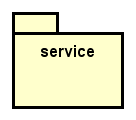
\includegraphics[scale=0.6]{img/RelationPackage/service}
	\caption{Package model::dataaccess::service}
	\label{servicePackage}
\end{figure}


\newpage
	\subsection{model::dataaccess::dao}
		Il package \verb|dao| è incaricato della costruzione dell'oggetto \verb|BuildingMap| attraverso altri componenti (\verb|-Table|) tramite i dati scaricati in formato Json o prelevati dal database SQLite locale. Il package è utilizzato solo dal package \verb|service| e le classi Factory sono utilizzate tramite la dependency injection.

\begin{figure}[h]
	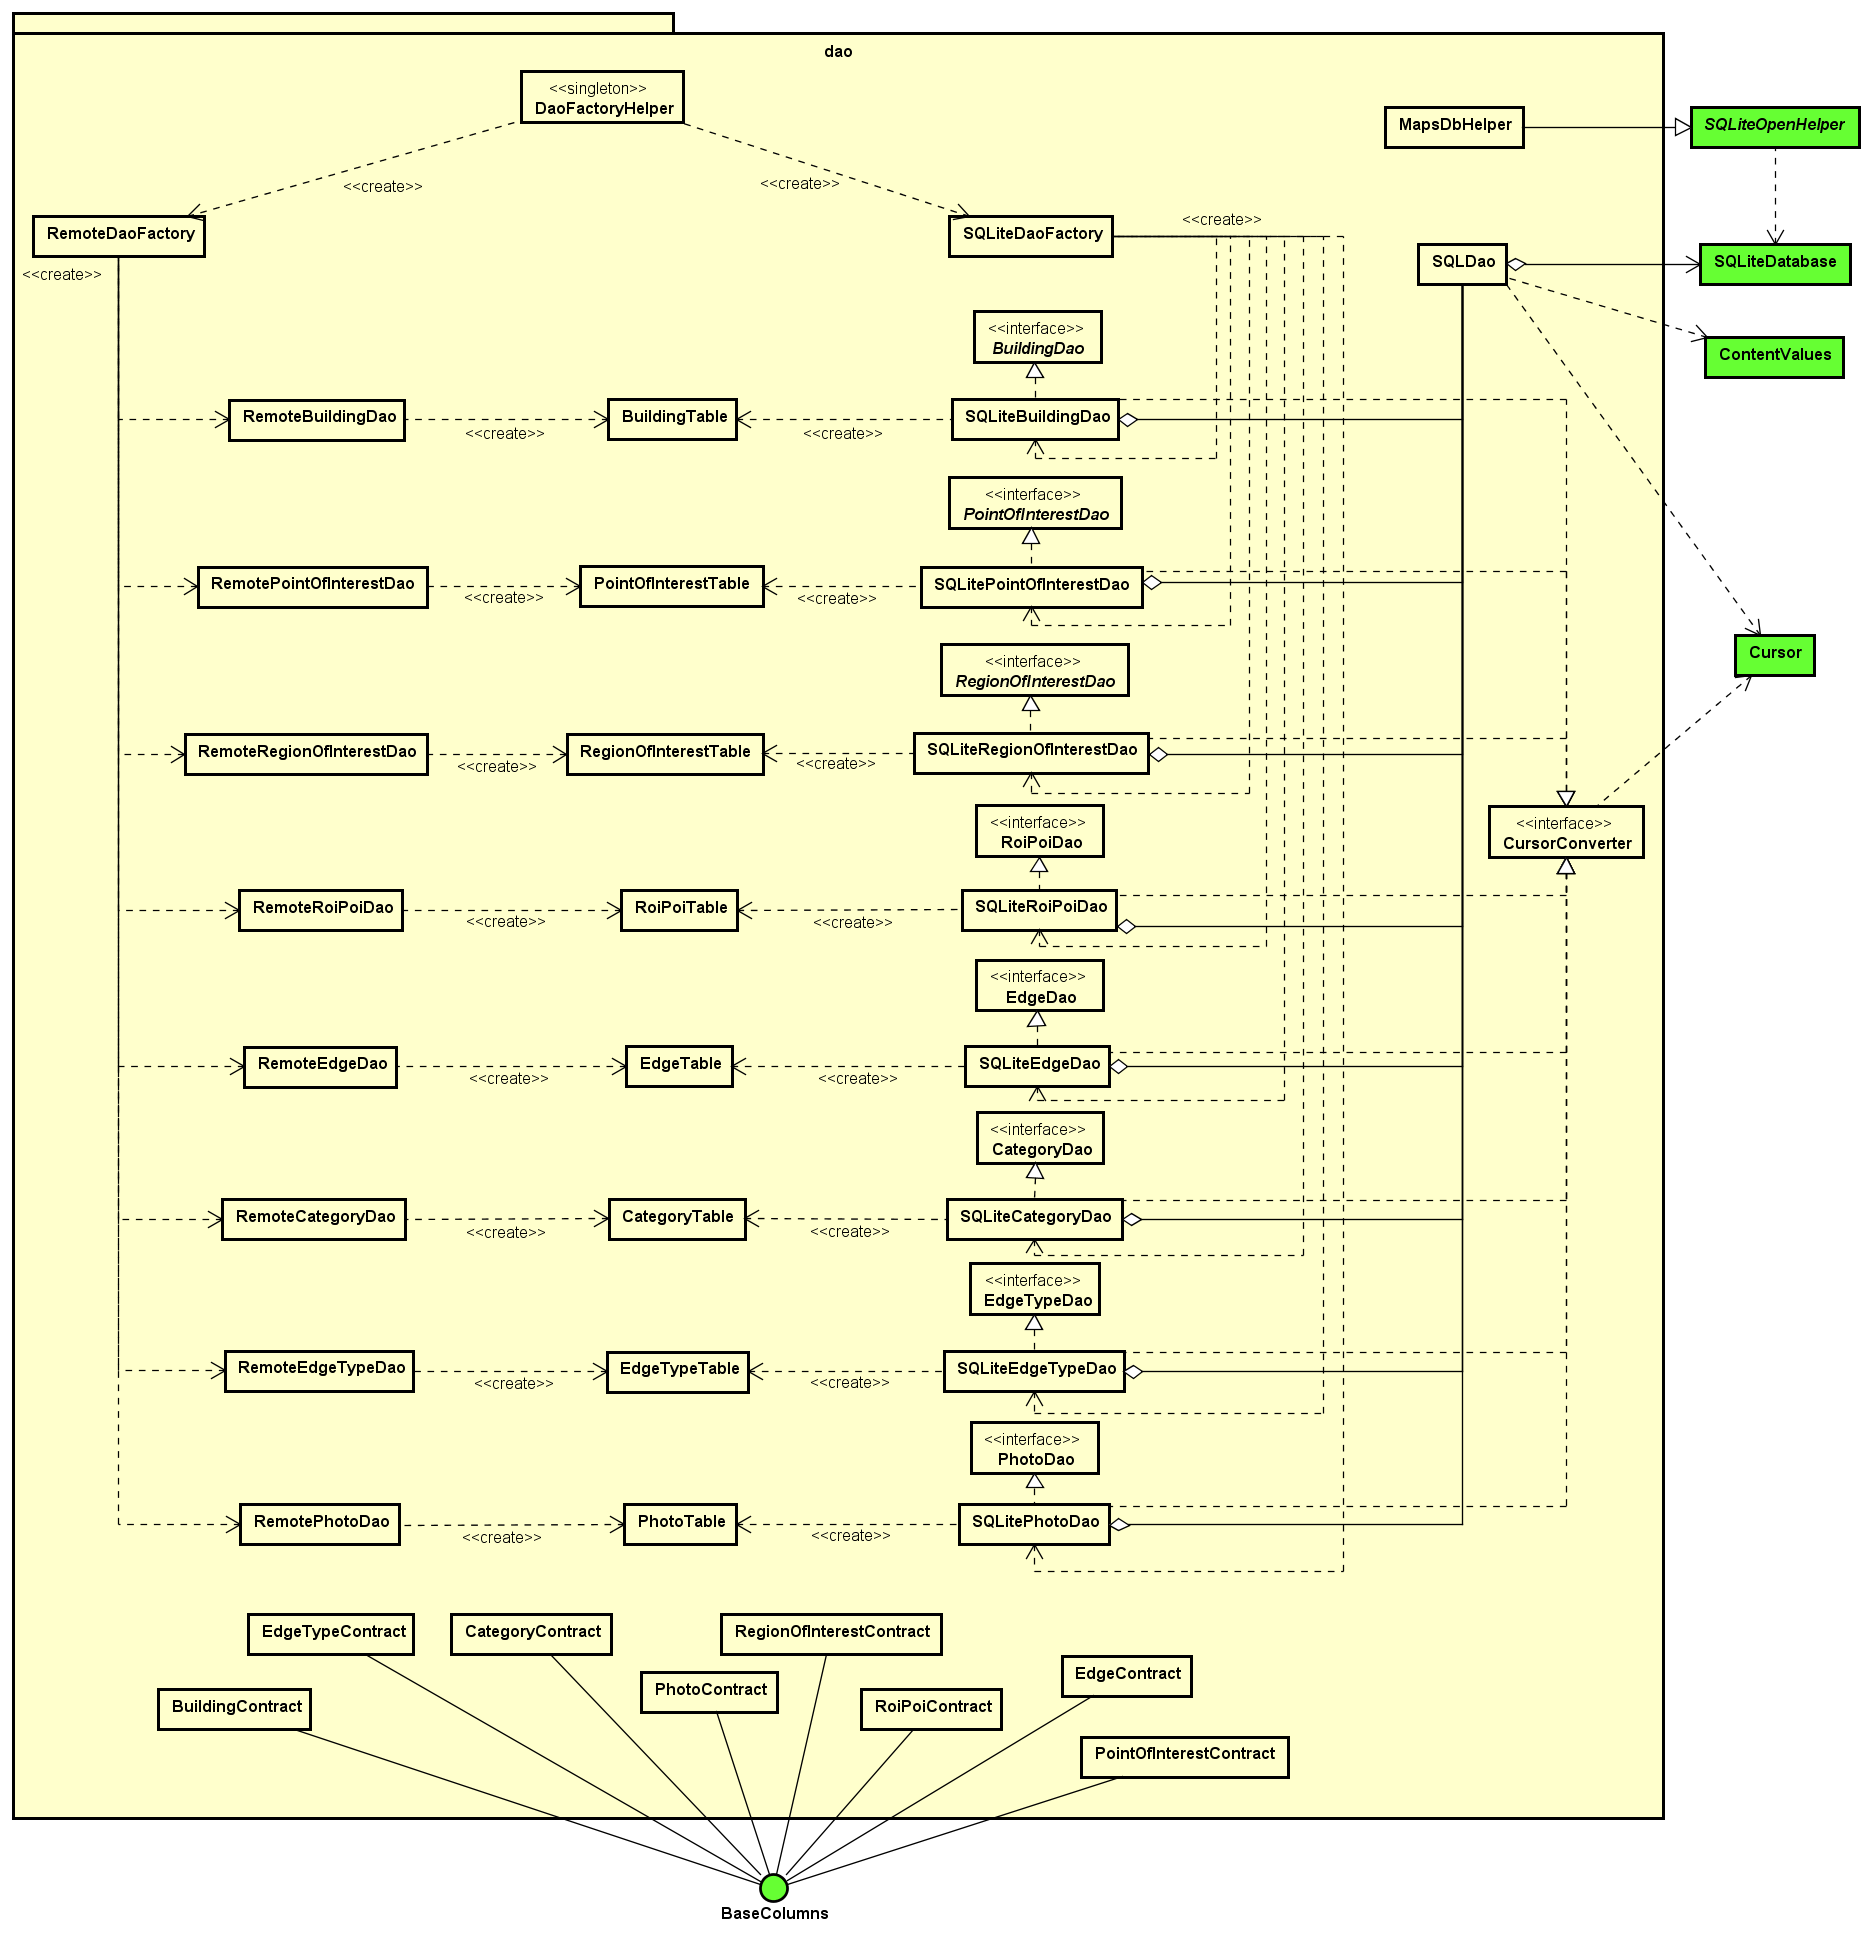
\includegraphics[width=\textwidth]{img/RelationPackage/dao}
	\caption{Package model::dataaccess::dao}
	\label{daoPackage}
\end{figure}


\newpage

	\subsection{model::navigator::graph}
		Il package \verb|graph| è incaricato di permettere la costruzione del grafo rappresentante l'edificio, l'oggetto \verb|MapGraph|. Esso è composto dai package: \verb|area|, \verb|navigationinformation|, \verb|edge| e \verb|vertex|.  Ha relazioni con il package esterno \verb|model| con la classe \verb|NavigationManagerImp| il quale contiene un campo \verb|MapGraph|.

\begin{figure}[h]
	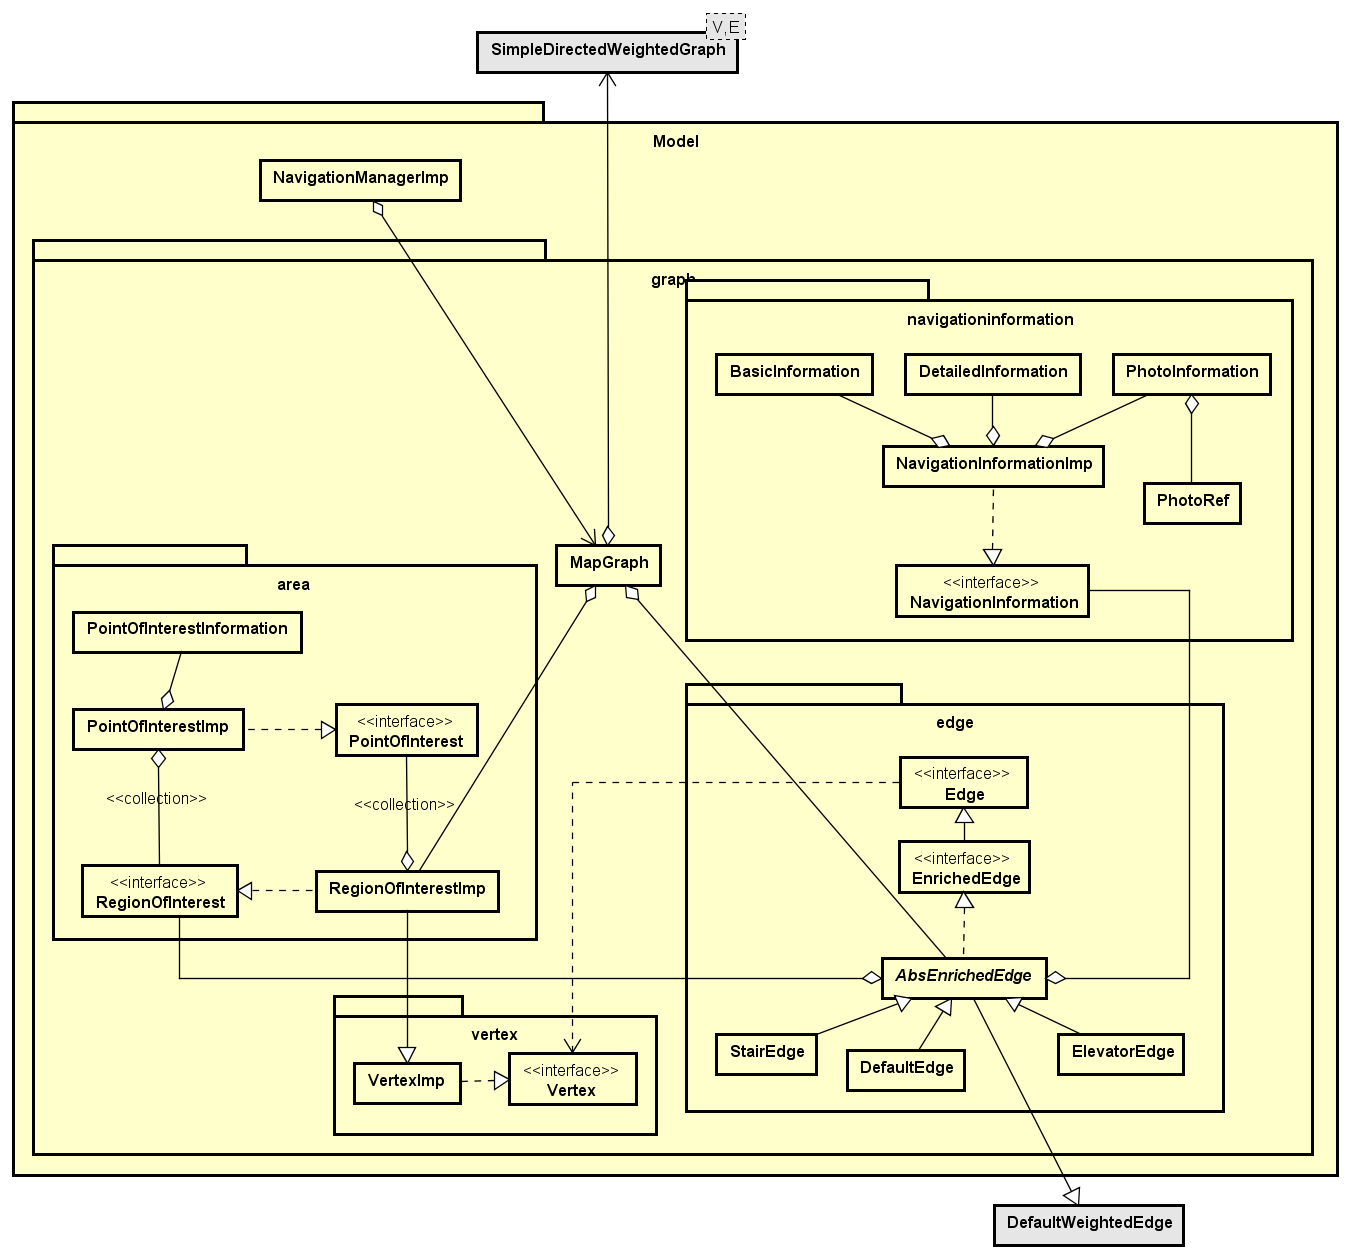
\includegraphics[width=\textwidth]{img/RelationPackage/graph}
	\caption{Package model::navigator::graph e relazioni con gli altri package}
	\label{graphPackage}
\end{figure}


\newpage
	
	\subsection{model::navigator}
		Il package \verb|navigator| ha il compito di eseguire i calcoli e di fornire le prossime istruzioni per permettere all'utente di navigare. Contiene il package \verb|graph| e \verb|algorithm|, quest'ultimo fornisce l'algoritmo di Dijkstra sul grafo fornito dal package \verb|graph|.

\begin{figure}[h]
	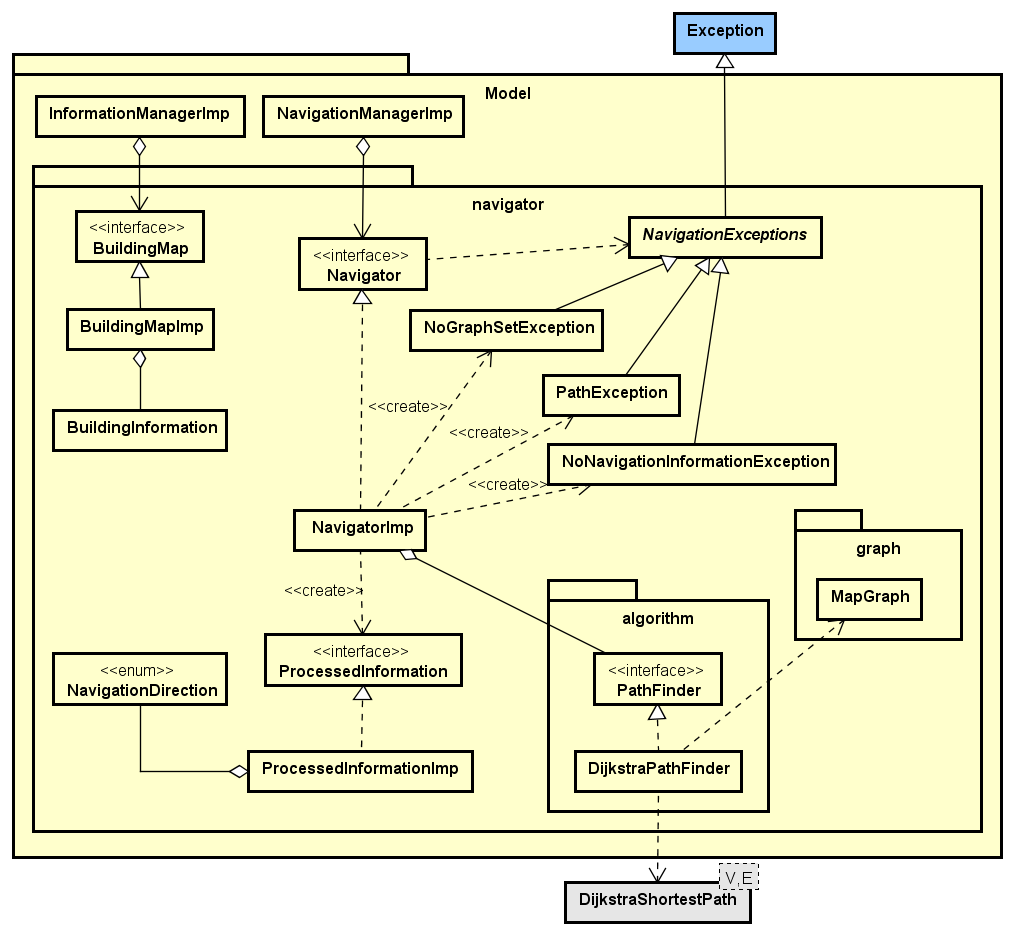
\includegraphics[width=\textwidth]{img/RelationPackage/navigator}
	\caption{Package model::navigator e relazioni con gli altri package}
	\label{navigatorPackage}
\end{figure}


\newpage

	\subsection{model::compass}
		Il package \verb|compass| ha il compito di calcolare l'orientamento del dispositivo fisico attraverso i dati ricavati dai sensori dello stesso. Esso attraverso l'uso di listener comunica direttamente con il \verb|presenter|.

\begin{figure}[h]
	\centering
	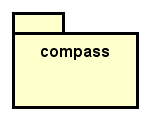
\includegraphics[scale=0.6]{img/RelationPackage/compass}
	\caption{Package model::compass e relazioni con gli altri package}
	\label{compassPackage}
\end{figure}


\newpage

	\subsection{model::usersetting}
		Il package \verb|usersetting| permette di utilizzare la funzionalità \verb|SharedPreference| offerta dall'SDK Android. Esso comunica solo con il package esterno \verb|model| che lo contiene.

\begin{figure}[h]
	\centering
	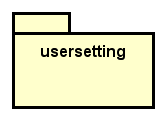
\includegraphics[scale=0.6]{img/RelationPackage/usersetting}
	\caption{Package model::usersetting e relazioni con gli altri package}
	\label{usersettingPackage}
\end{figure}


\newpage
	\subsection{model::beacon}
		Il package \verb|beacon| permette l'utilizzo della libreria AltBeacon per interfacciarsi con la tecnologia beacon. Il package comunica con il package esterno, il \verb|model|, attraverso l'uso degli \verb|Intent| offerti dall'SDK Android attraverso i quali vengono passati oggetti \verb|MyBeaconImp|.

\begin{figure}[h]
	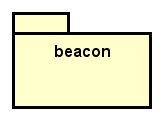
\includegraphics[width=\textwidth]{img/RelationPackage/beacon}
	\caption{Package model::beacon e relazioni con gli altri package}
	\label{beaconPackage}
\end{figure}


\newpage
	\subsection{model}
		Il package \verb|model| contiene tutta la business logic dell'applicazione che è gestita attraverso le due classi principali \verb|InformationManager| e \verb|NavigationManager|. Esse sono incaricate della gestione di tutte le sottocomponenti e della comunicazione con il \verb|presenter|.

\begin{figure}[h]
	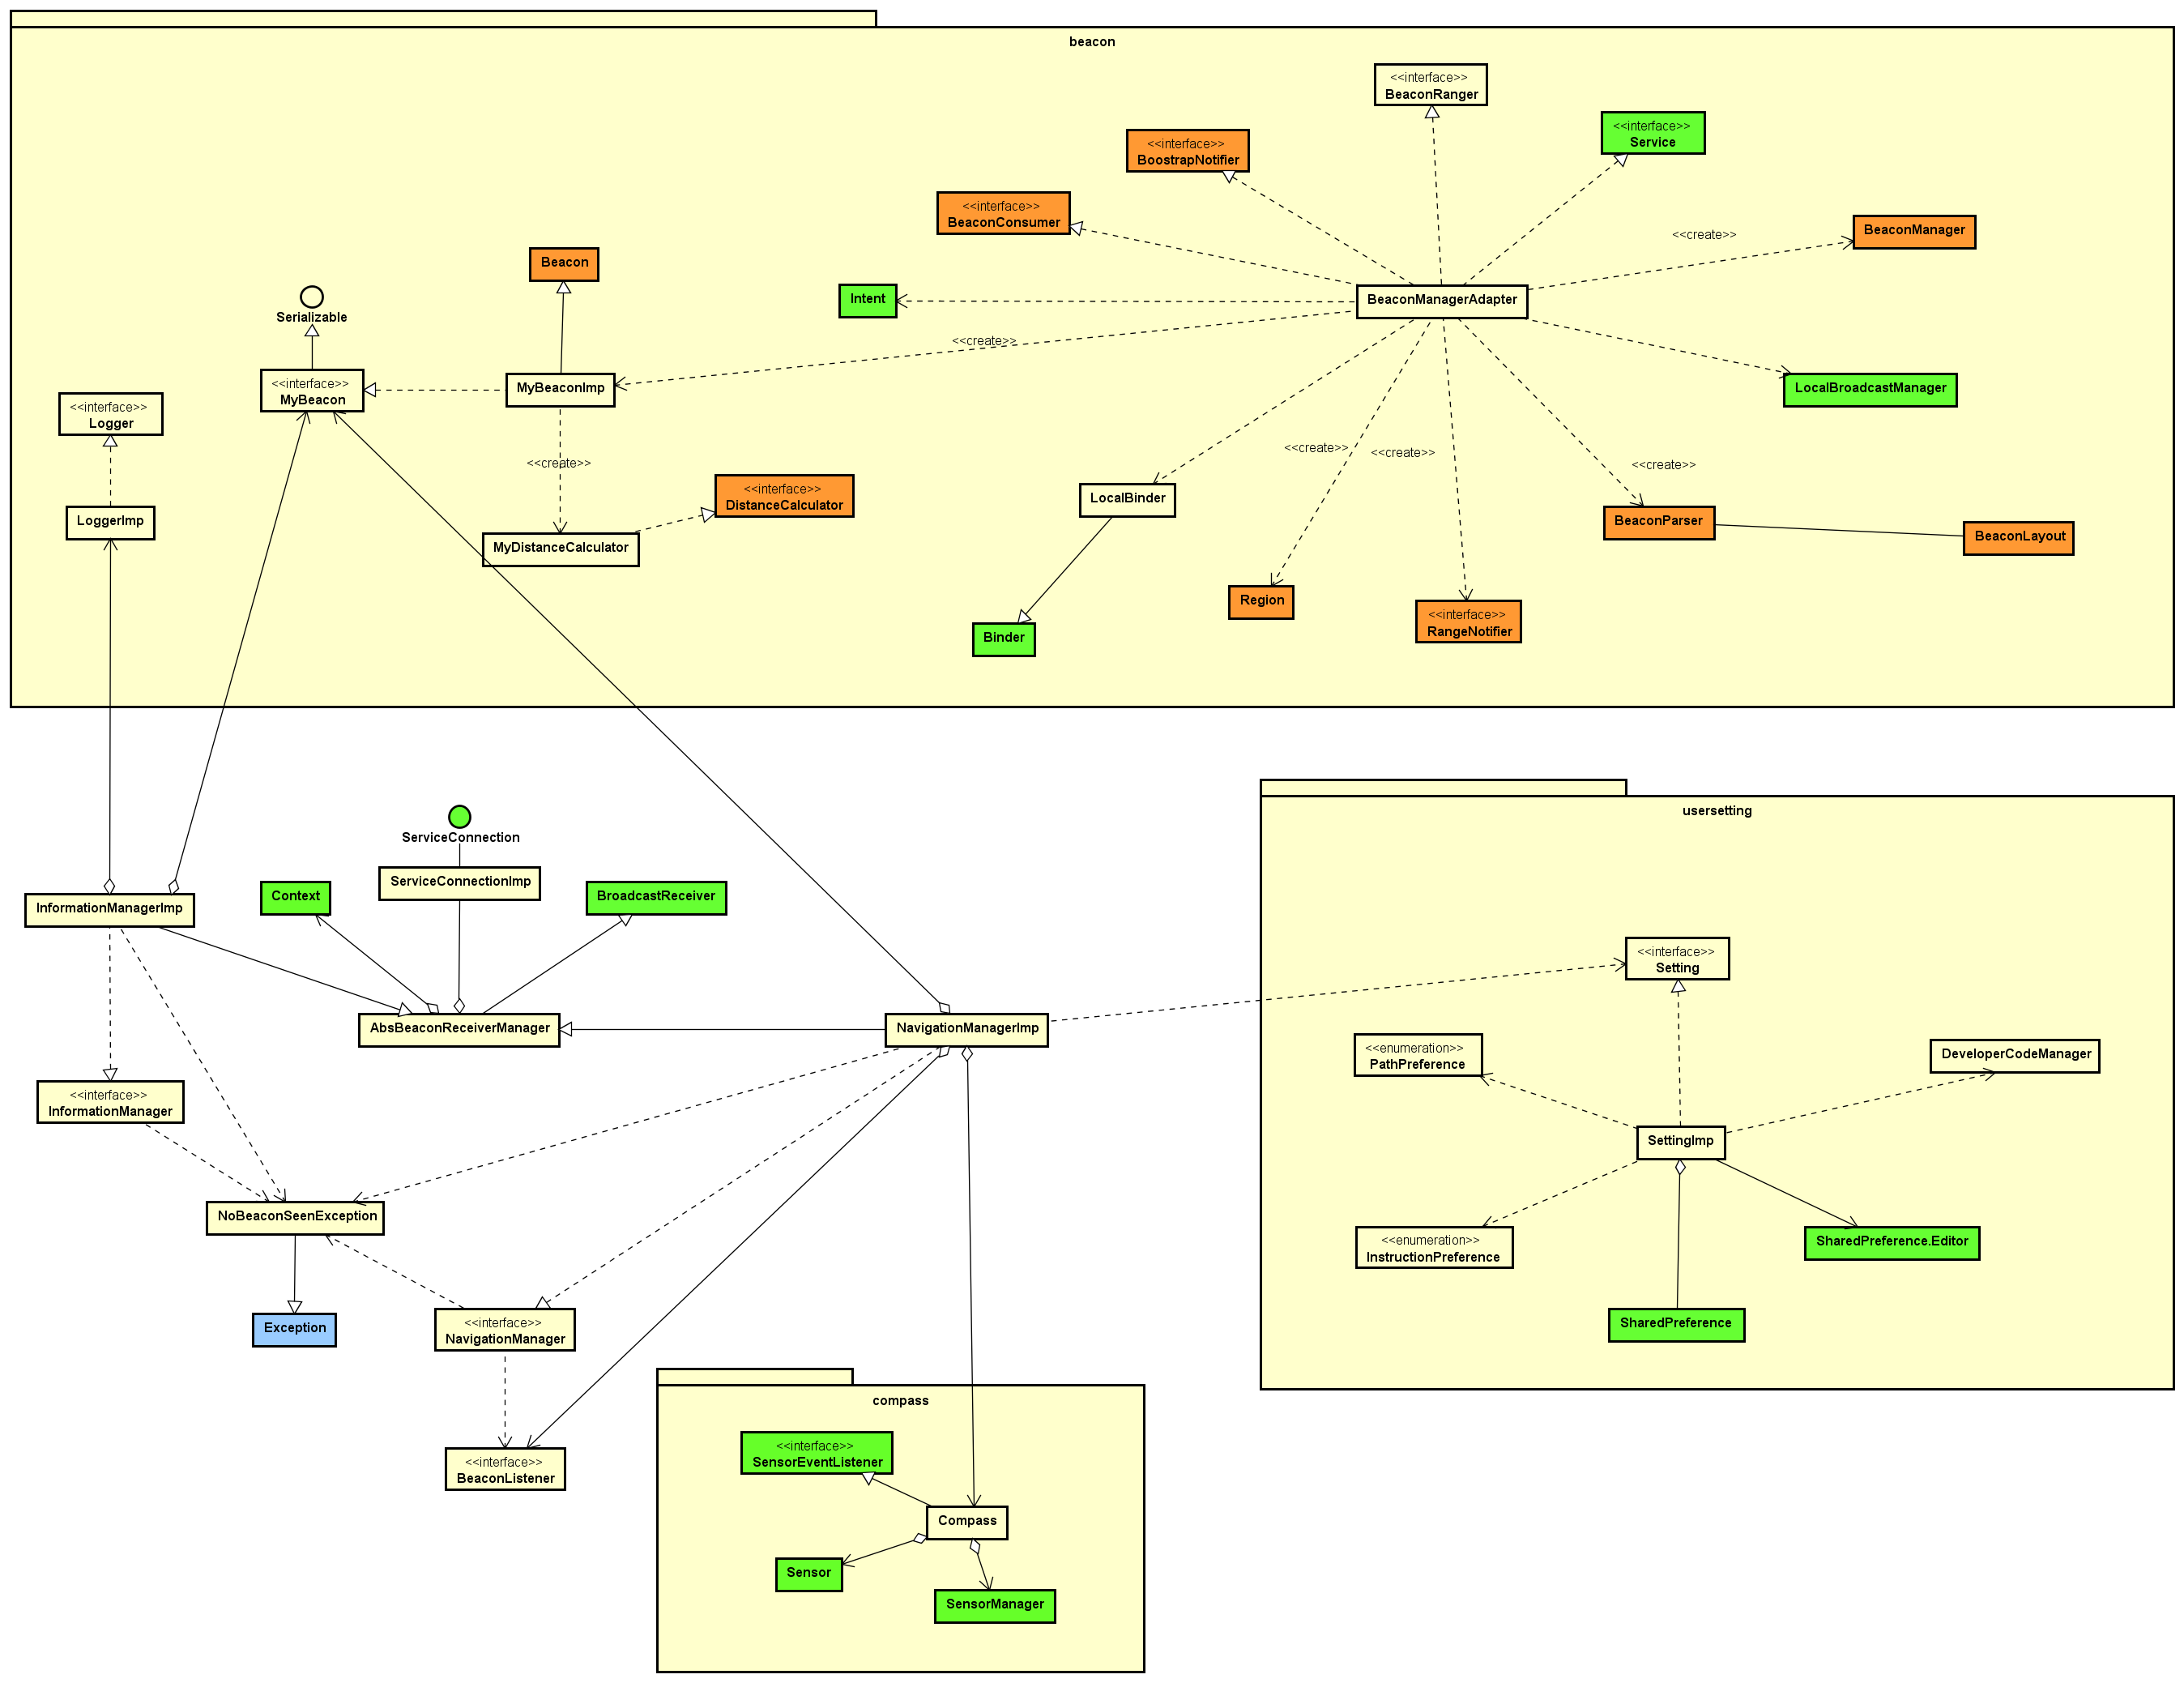
\includegraphics[width=\textwidth]{img/RelationPackage/model}
	\caption{Package model e relazioni con i package interni}
	\label{modelPackage}
\end{figure}

\newpage
	\subsection{presenter}
	
	
\begin{figure}[h]
	\centering
	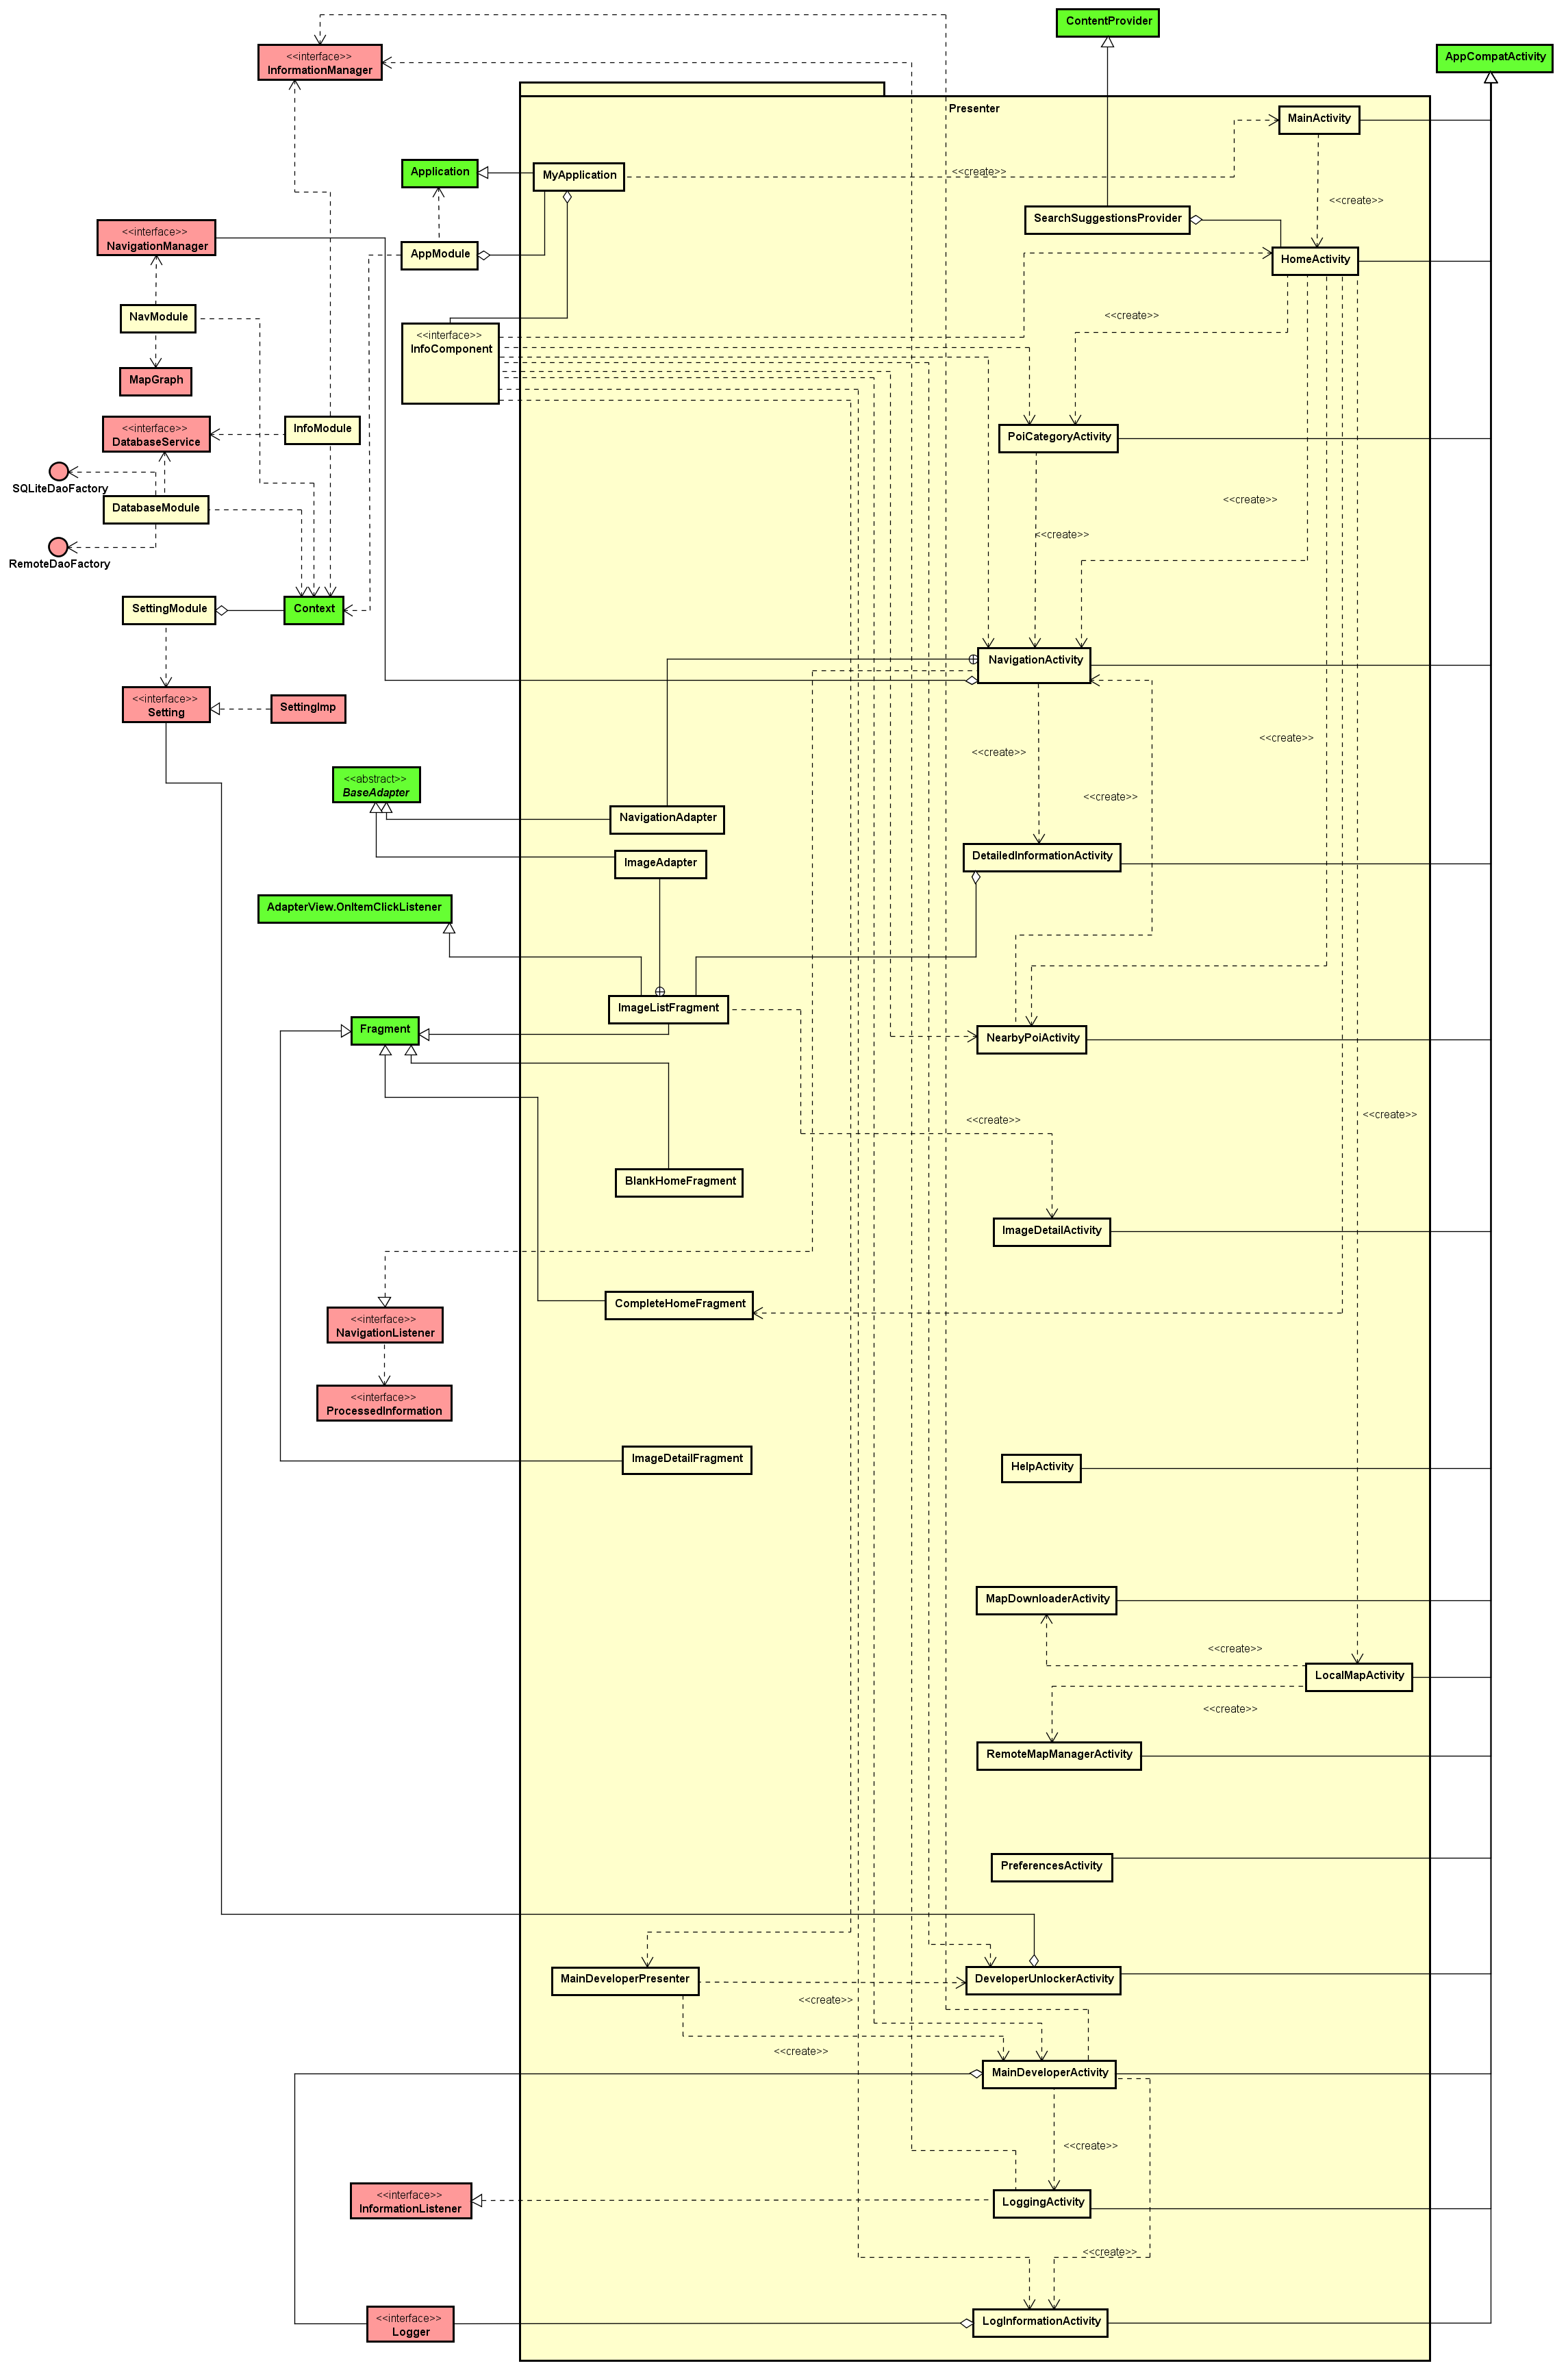
\includegraphics[height=0.9\textheight, width=\textwidth, keepaspectratio]{diagrams/ModelCompleteNoMethods/PNGpackage/presenter}
	\caption{Package presenter e relazioni con le componenti del package view}
	\label{presenterPackage}
\end{figure}


\newpage
	\subsection{view}
		Il package

\begin{figure}[h]
	\centering
	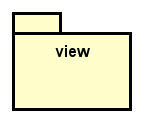
\includegraphics[height=0.9\textheight, width=\textwidth, keepaspectratio]{diagrams/ModelCompleteNoMethods/PNGpackage/view}
	\caption{Package view e relazioni con le componenti del package presenter}
	\label{viewPackage}
\end{figure}


\begin{figure}[p]
	\centering
	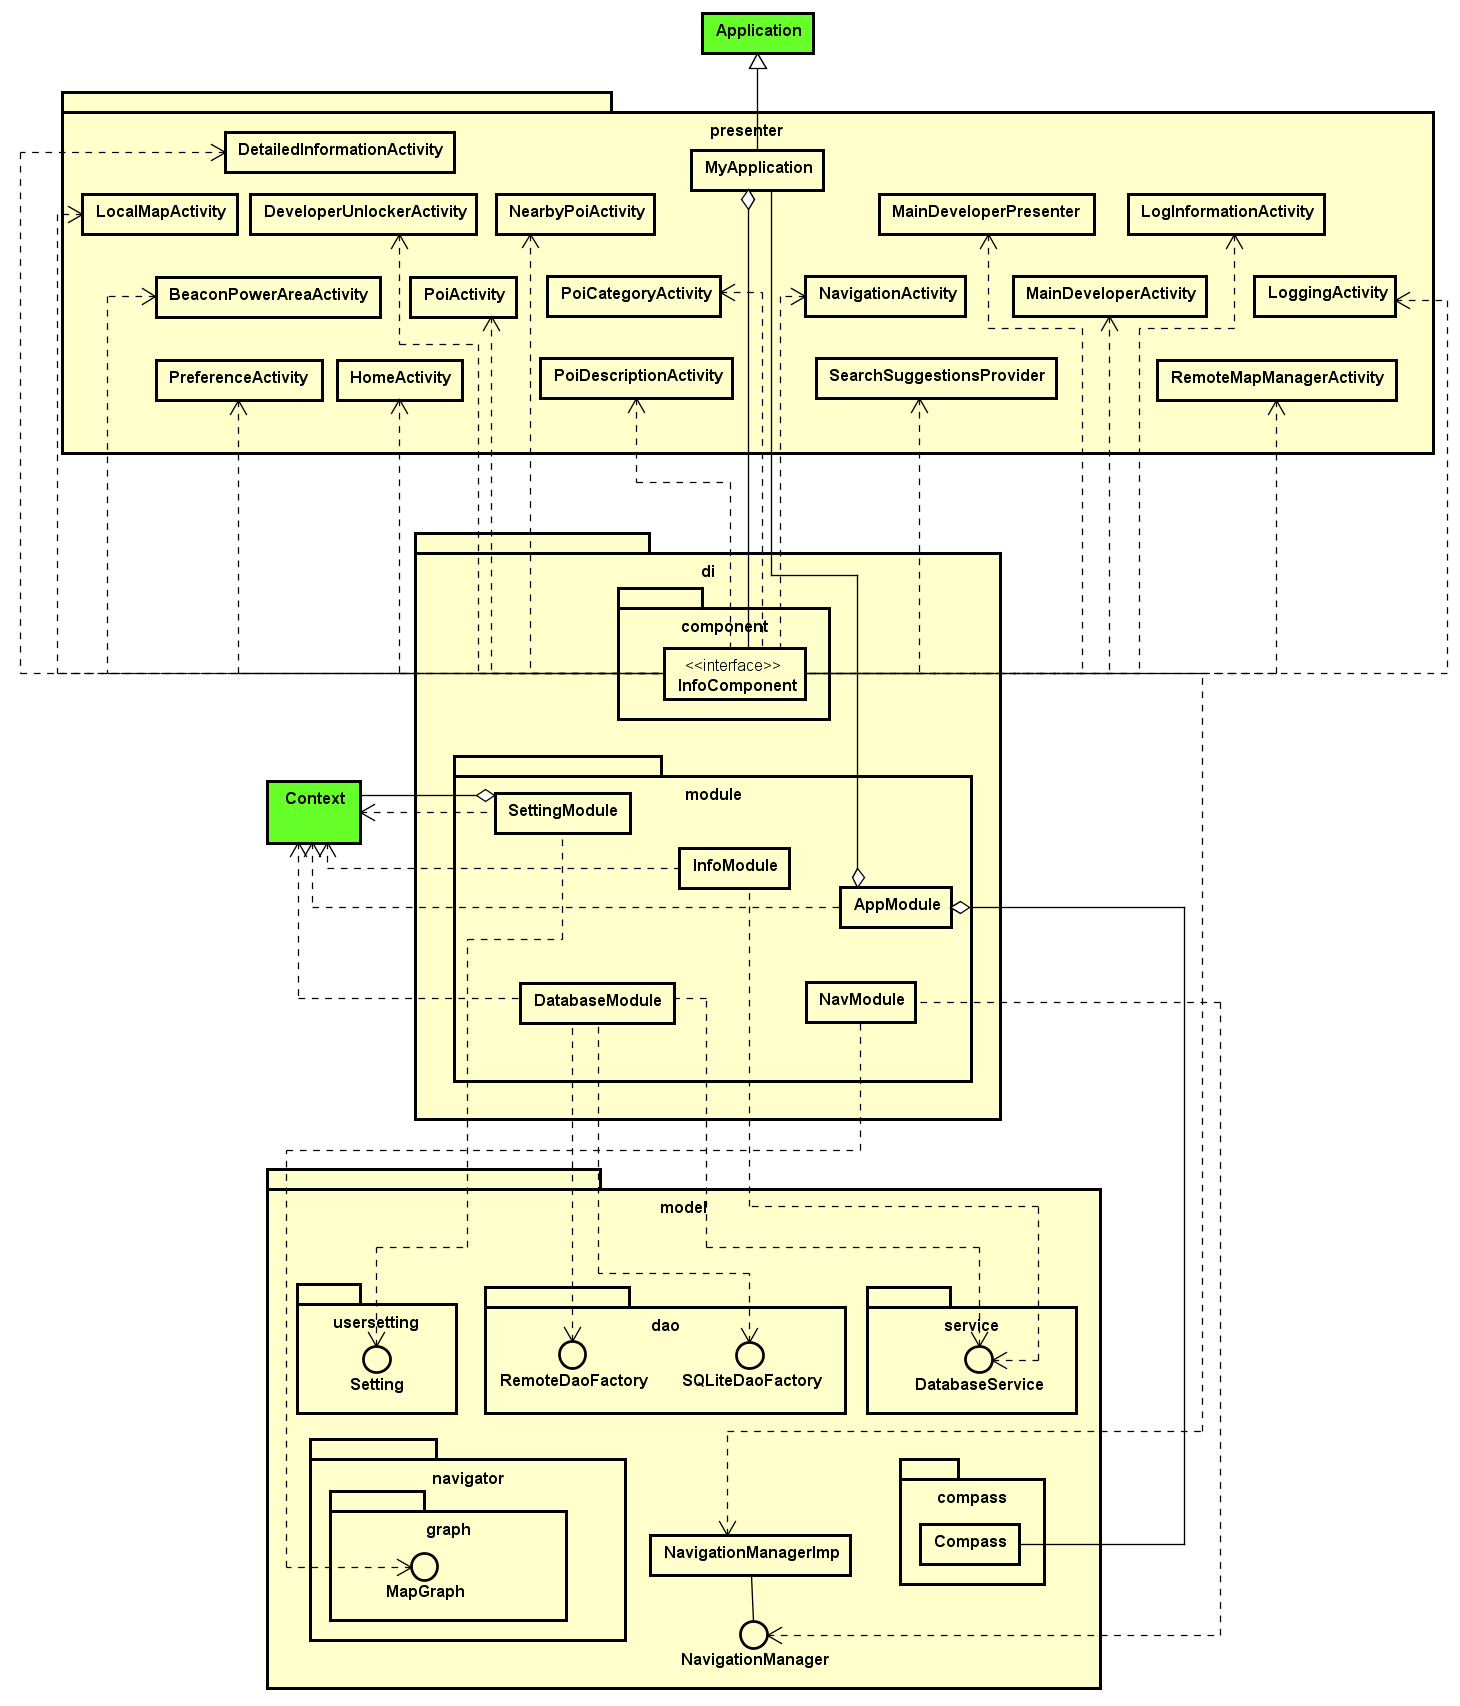
\includegraphics[height=19cm,width=\textwidth]{diagrams/ModelCompleteNoMethods/PNGpackage/di}
	\caption{Package di e relazioni con gli altri package}
	\label{diPackage}
\end{figure}

\end{document}